\documentclass[12 pt]{article}
\usepackage{fancyhdr}
\usepackage[margin = 1 in]{geometry}
\usepackage{amsmath}
\usepackage{enumerate}
% \usepackage{indentfirst}
\pagestyle{fancy}
\usepackage{graphicx}
\usepackage[version=3]{mhchem}
\fancyhf{}
\usepackage{sectsty}	
\lhead{Andrew Wang}
\chead{CS/CNS/EE 155 Machine Learning \& Data Mining}
\rhead{Yue}
\sectionfont{\fontsize{15}{18}\selectfont}
\usepackage{graphicx}
\usepackage{array}
\newcolumntype{P}[1]{>{\centering\arraybackslash}p{#1}}
\newcolumntype{M}[1]{>{\centering\arraybackslash}m{#1}}
\usepackage[font=small,labelfont=bf]{caption}
\usepackage{float}
\usepackage{float}
\usepackage{subfig}
\usepackage{microtype}
\usepackage{ amssymb }
\usepackage{amsmath}
\usepackage{commath}
\begin{document}
	\begin{center}
		\section*{Homework 5}
	\end{center}
	
	
	\subsection*{1 Naive Bayes}	
	\textbf{Question A:}  \\
	For the Red Domestic SUV: \\
	
	\noindent \begin{eqnarray*}
	&& P(\text{stolen}) \prod P(a_i | v_j) \\
	&=& P(\text{stolen}) P(\text{Red}|\text{stolen}) P(\text{SUV}|\text{stolen}) P(\text{Domestic}|\text{stolen}) \\
	&=& \frac{3}{10}  \cdot \frac{4.5}{6}\cdot \frac {3.5}{6} \cdot \frac {1.5}{6}   \\
	&=& 21/640 = 0.0328125\\
	\\
	&& P(\text{not stolen}) \prod P(a_i | v_j) \\
	&=& P(\text{not stolen}) P(\text{Red}|\text{not stolen}) P(\text{SUV}|\text{not stolen}) P(\text{Domestic}|\text{not stolen}) \\
	&=& \frac{7}{10}  \cdot \frac{3.5}{10}\cdot \frac {5.5}{10} \cdot \frac {4.5}{10}   \\
	&=& 4851/80000 = 0.0606375
	\end{eqnarray*} 

	\noindent The resulting V$_{nb}$ = 0.0606375, and my Red Domestic SUV car is more likely not to be stolen than stolen. \\

	\noindent\textbf{Question B:}  \\
	No, Naive Bayes should not be used. Naive Bayes makes the assumption that the features are strongly independent of one another. In this case, we can clearly see that how much one sleeps one day most definitely affects how much one sleeps the next day and so forth. Thus, the assumption is invalid in this case.
 
	
	\subsection*{2 Sequence Prediction}
	\noindent\textbf{Question A:} \\
	The naive algorithm has time complexity O(L$^M$) where L is the number of possible states, and M is the length of the sequence.\\
	
	\noindent\textbf{Question B:} \\ The Viterbi algorithm has time complexity O(M $\cdot$ $|$L$|$$^2$).\\

	%\begin{figure}[h]
	%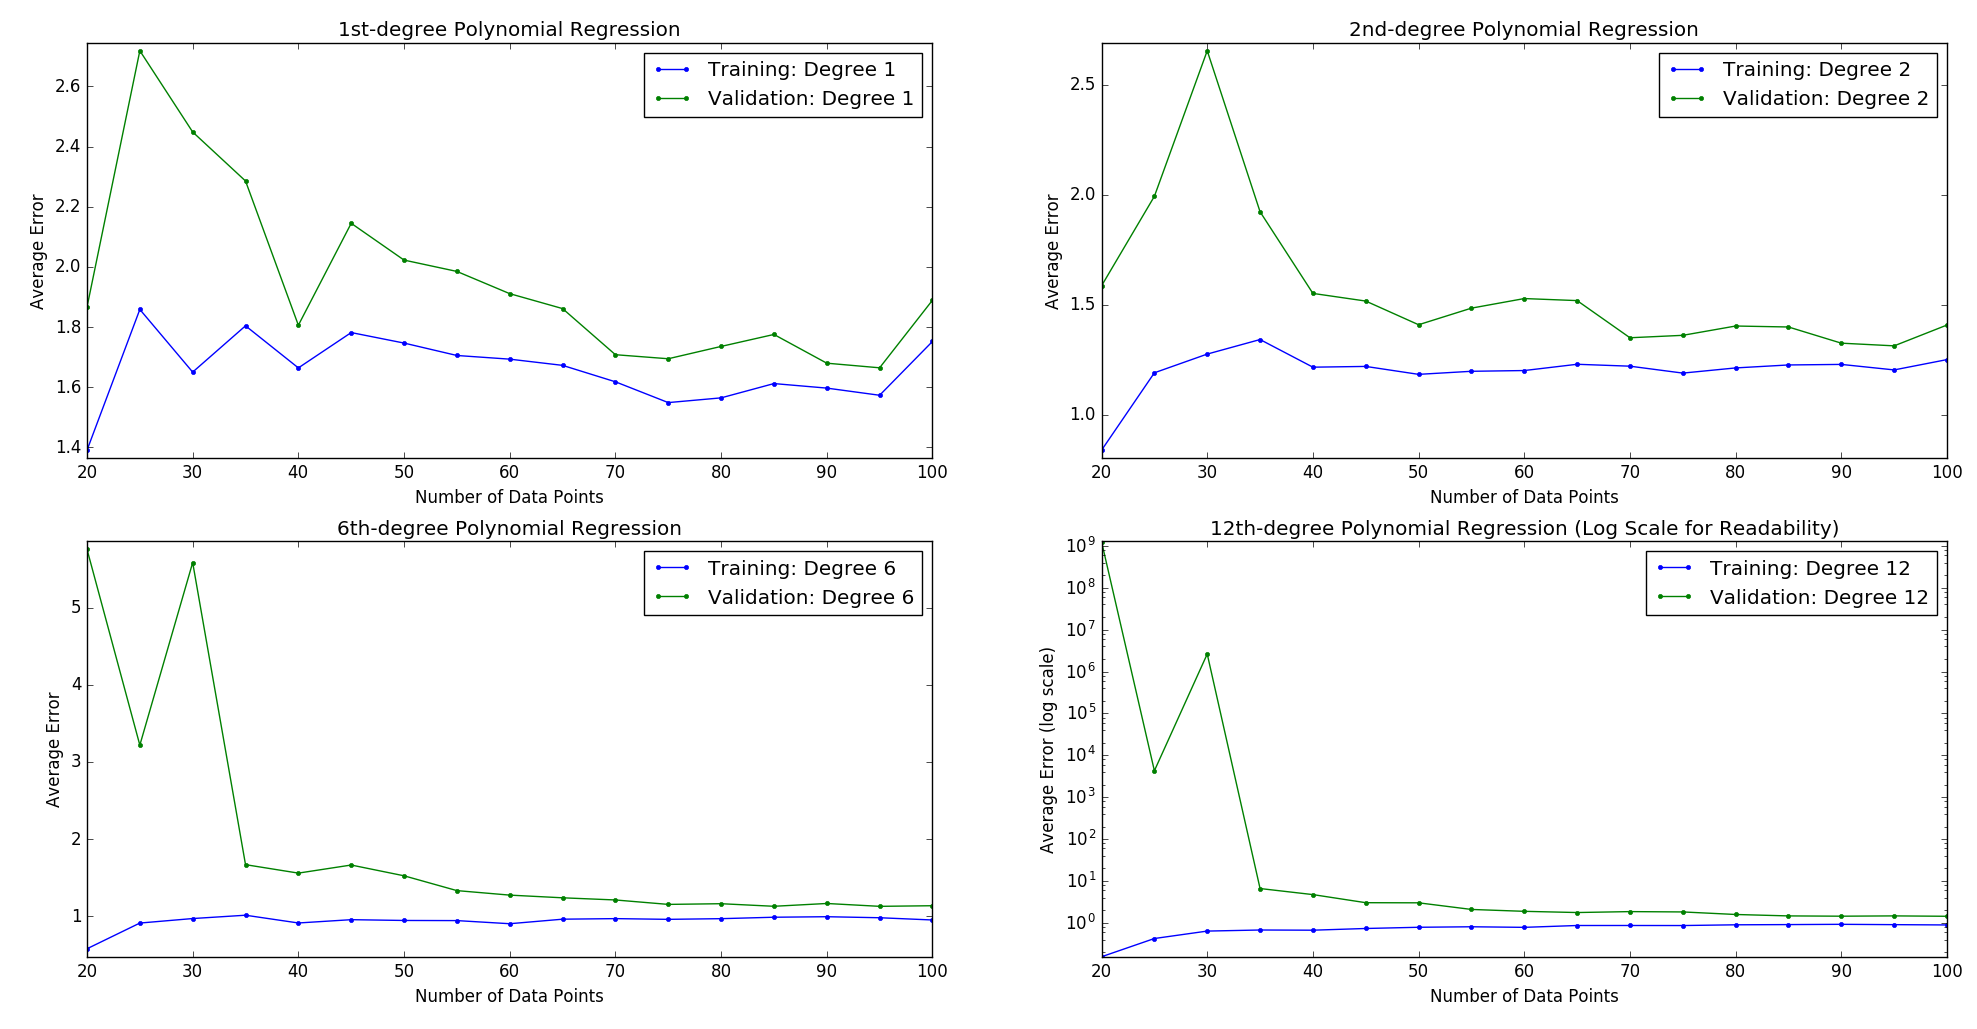
\includegraphics[width=17cm]{LearningCurves}
	%\end{figure}	
	
	\noindent\textbf{Question C:}  True. When we increase the number of hidden states, it is essentially increasing the number of possibilities we have for classifying the observation. We take the speech example presented in lecture. If we have a limited amount of hidden states (parts of speech) such that the input sequence consists of words that if correctly labeled, would fall into hidden states/ parts of speech not in our current HMM, then the likelihood would be very low. However, if we add more hidden states/ parts of speech into our HMM such that the words in our limited HMM can now be correctly classified, the likelihood increases.  \\
	
	\noindent\textbf{Question D:} \\
	\noindent From lecture slides, recall that $\alpha_z(1) = P(y^1 = z \;|\; y^0) P(x^1 \;| \;y^1 = z)$. If some coefficient of initial state is initially 0, then we get that for some z, $P(y^1 = z) = 0$ which then means that $P(y^1 = z \;|\; y^0) = 0$, and thus $\alpha_z$(1) = 0. Now, recall that our initial state distribution and transition matrix are updated as follows:
	
	\begin{figure}[H]
		\centering
	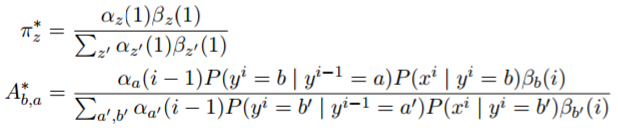
\includegraphics[width=10cm]{equations}
	\end{figure}	

	\noindent Because $\pi^*_z$ relies on $\alpha_z$(1), $\pi^*_z$ = 0 when $\alpha_z$(1) = 0 and if any coefficient of the initial state is initially 0, it will remain 0. \\
	
	\noindent Similarly, if the coefficient of the state transition probability of a HMM is initially 0, then $P(y^i = b \;|\; y^{i-1} = a) = 0$ for that specific transition. Note that this term is included in the numerator of the transition matrix so if $P(y^i = b \;|\; y^{i-1} = a) = 0$, then $A^*_{b,a}$ = 0 and thus the transition probabilities will not be updated. Hence, if a coefficient of the state transition probability matrix is initially 0, it will remain 0.
	\\
	
	
	\noindent\textbf{Question E:} \\
	\begin{figure}[H]
	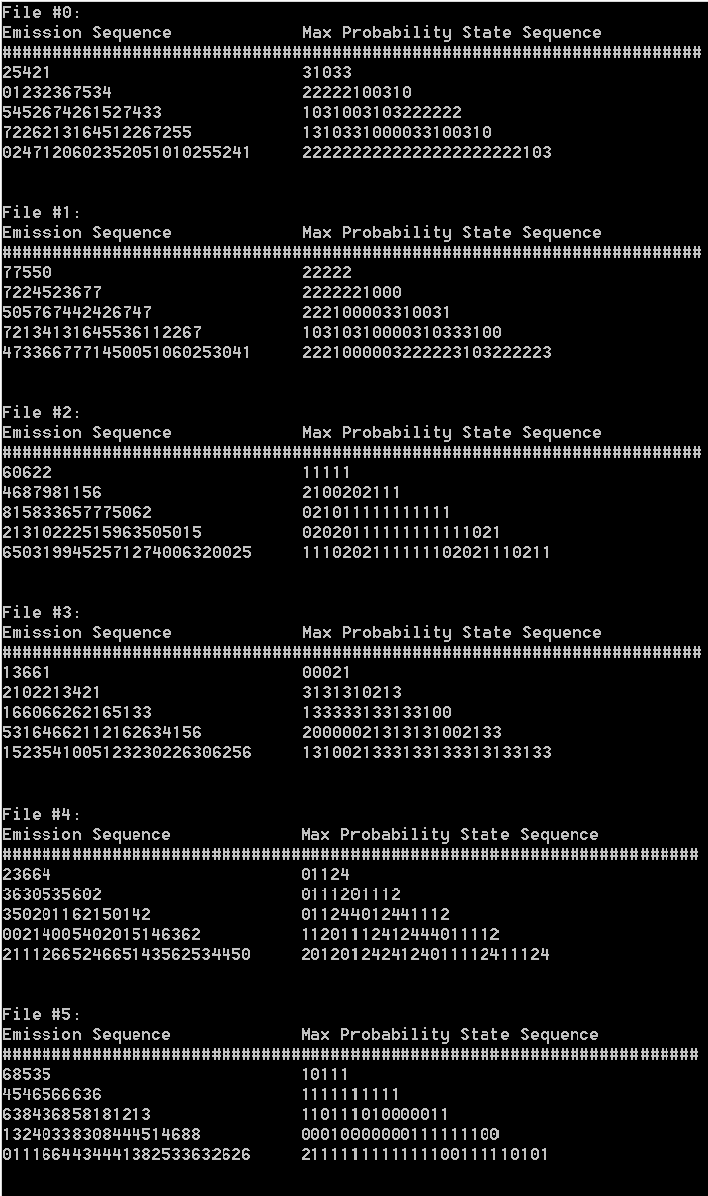
\includegraphics[width=13cm]{2E}
	\end{figure}
	
	\noindent\textbf{Question F:} \\
	\noindent\textbf{i.}
	\begin{figure}[H]
		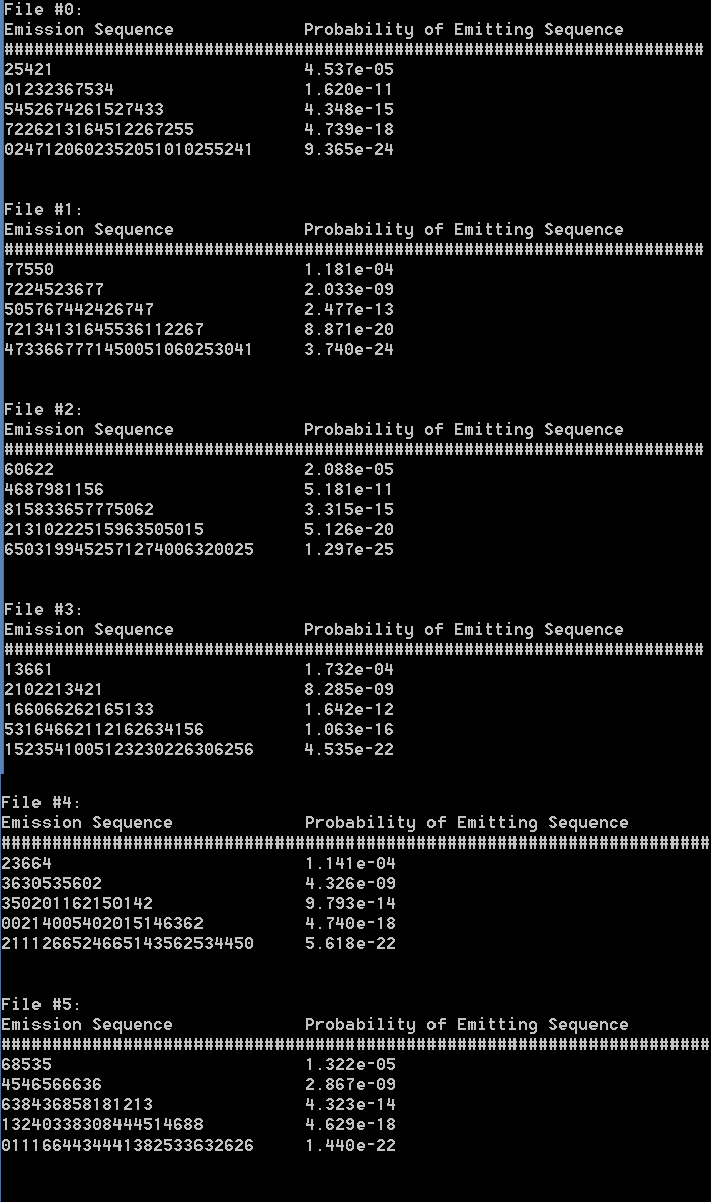
\includegraphics[width=13cm]{2Fi}
	\end{figure} 
	
	\noindent\textbf{ii.}
	\begin{figure}[H]
	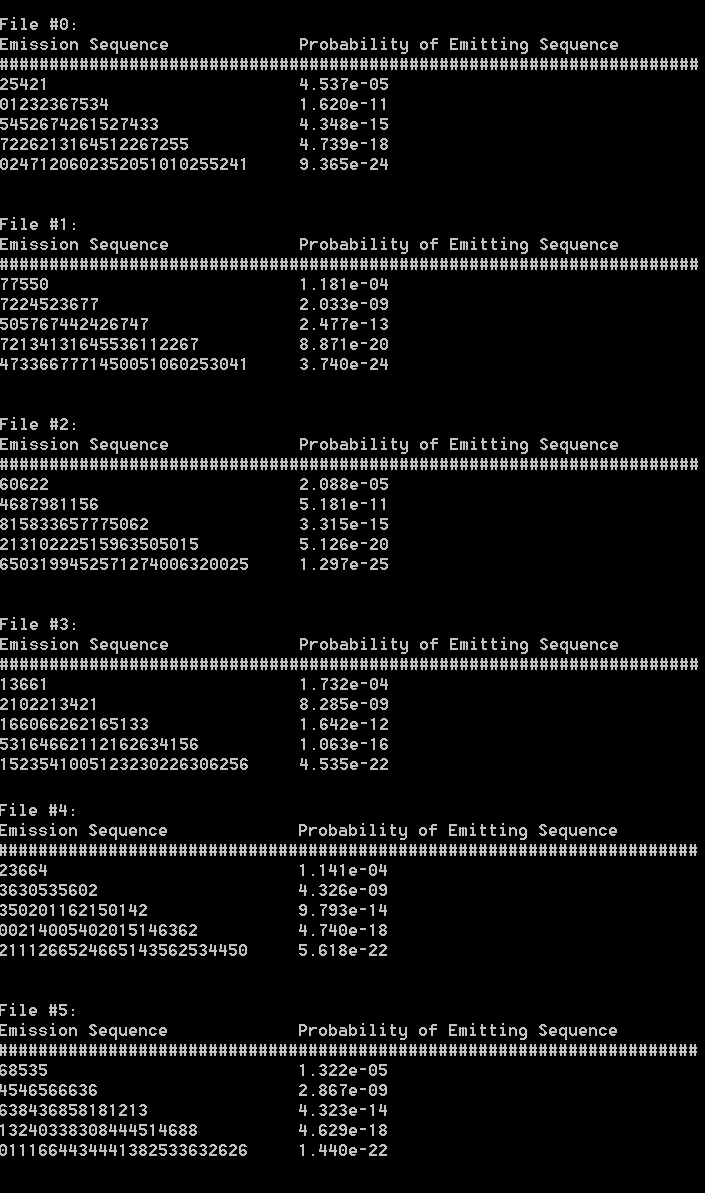
\includegraphics[width=13cm]{2Fii}
	\end{figure} 
	
	\noindent\textbf{Question G:} 
	
	\begin{figure}[H]
		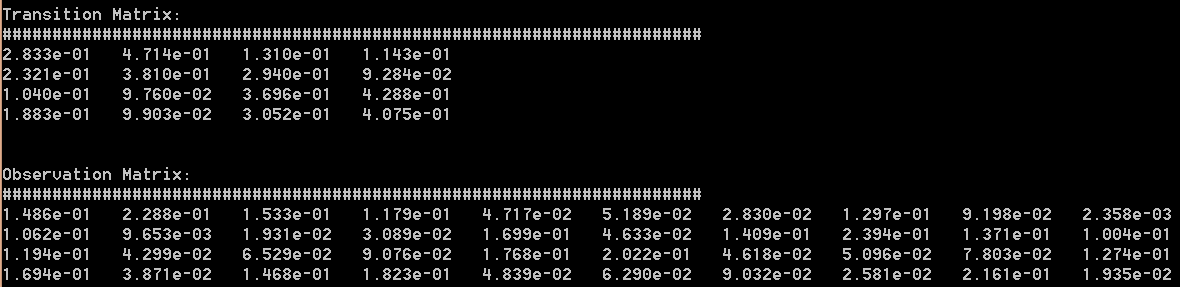
\includegraphics[width=16cm]{2G}
	\end{figure} 

	\noindent\textbf{Question H:} 
	\begin{figure}[H]
	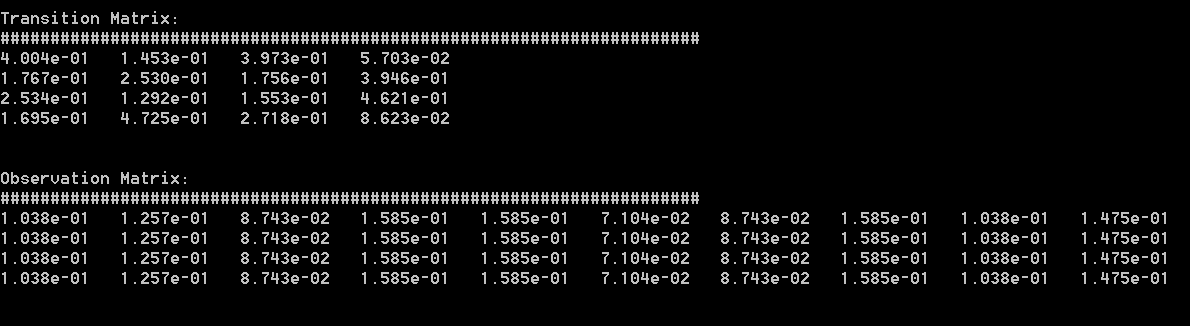
\includegraphics[width=\linewidth]{2H}
	\end{figure} 

	\noindent\textbf{Question I:}
	\noindent It seems that the matrices from 2G provide a more accurate representation  of Ron's mood and how they affect his music choices. First of all, 2G is trained with fully supervised data while 2H is trained with unsupervised data(half of data in 2G). It makes intuitive sense that when given the moods of training data, we are better able to make predictions on moods than if we did not have these labels. Moreover, patterns in unsupervised learning is generally harder to decipher because there is a tendency to go to a local minimum which may not be meaningful.\\
	
	 \noindent Also, in comparing the transition matrices, we see that a majority of the values lying on the principal diagonal for 2G are greater than the corresponding diagonal values of 2H. These values correspond to the probabilities of staying in a current mood. Not an expert on human behavior, but it does seem that moods tend to linger. In addition, looking at the observation matrix for 2H and the same values for each column, it's unlikely that an observation (song choice)is equally likely for all states (moods).\\
	 
	 \noindent One way to improve the unsupervised method is to increase the training data set by getting more observations.\\
	 
	 \noindent\textbf{Question J:} My favorite sequence is the second of file $\#$5. It reads "84883333312318283228." This is my favorite because it's essentially dominated by the two numbers, 8 and 3, a level of domination by two digits that is hard to see in the other generated emissions.\\
	 \begin{figure}[H]
	 	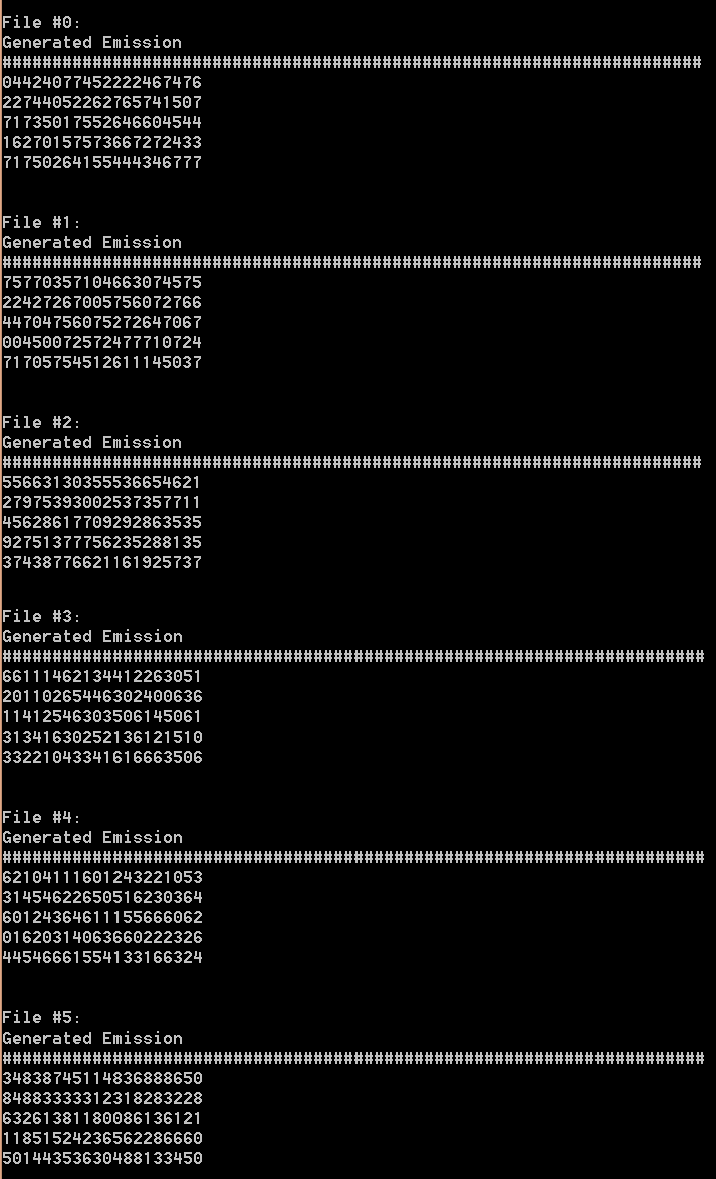
\includegraphics[width=13cm]{2J}
	 \end{figure} 


	
\end{document}